\documentclass[a4paper]{article}

\title{Дифференцирование и интегрирование сигналов}
\author{Бояринцева Н.А. \and Можаров А.Р.}
\date{26 ноября 2023}

\usepackage{cmap}
\usepackage[T2A]{fontenc}
\usepackage[utf8]{inputenc}
\usepackage[russian]{babel}
\usepackage{indentfirst}
\usepackage[hidelinks]{hyperref}
\usepackage{circuitikz}
\usepackage{pgfplots}
\usepackage{amsmath}
\usepackage{amssymb}
\usepackage{subcaption}
\usepackage{comment}
\usepackage{xcolor}

\renewcommand{\thesubfigure}{\arabic{figure}.\arabic{subfigure}}
\DeclareCaptionLabelFormat{My}{Рис. #2: }
\captionsetup[subfigure]{labelformat=My}

\begin{document}

\maketitle

\section*{\centering Теоретическая часть}

\subsection*{Четырёхполюсники}

Под {\it четырёхполюсником} понимается электрическая цепь,
имеющая четыре наружных контакта,
с помощью которых она подключается к другим цепям.
Как правило, имеет смысл одну пару контактов называть входными,
а другую выходными.

Если на вход четырёхполюсника подаётся сигнал $U_\text{вх.}(t)$,
то с выхода дифференцирующего четырёхполюсника ожидается сигнал:
\begin{gather*}
    U_\text{вых.}(t) = \tau_0 \cdot \dfrac{dU_\text{вх.}(t)}{dt}
\end{gather*}
а с интегрирующего сигнал:
\begin{gather*}
    U_\text{вых.}(t) = \dfrac{1}{\tau_0} \int\limits_{-\infty}^{t} U_\text{вх.}(\tau)d\tau
\end{gather*}
где $\tau_0$ --- константа, имеющая размерность времени,
называемая {\it постоянной времени}.

\begin{figure}
    \centering
    \begin{subfigure}{0.45\textwidth}
        \centering
        \begin{circuitikz}[european resistors, american inductors]
            \draw (0, 0.5) to [short, o-] (0, 1) to [C, l=$C$, -*] (2, 1)
            to [R, l=$R$, -*] (2, -1) -- (0, -1) to [short, -o] (0, -0.5);
            \draw (2, 1) -- (3.5, 1) to [short, -o] (3.5, 0.5);
            \draw (2, -1) -- (3.5, -1) to [short, -o] (3.5, -0.5);
            \draw (0, 0) node[open]{$U_\text{вх.}$};
            \draw (3.5, 0) node[open]{$U_\text{вых.}$};
        \end{circuitikz}
        \caption{Дифференцирующий четырёхполюсник}
        \label{Дифференцирующий четырёхполюсник}
    \end{subfigure}
    \begin{subfigure}{0.45\textwidth}
        \centering
        \begin{circuitikz}[european resistors, american inductors]
            \draw (0, 0.5) to [short, o-] (0, 1) to [R, l=$R$, -*] (2, 1)
            to [C, l=$C$, -*] (2, -1) -- (0, -1) to [short, -o] (0, -0.5);
            \draw (2, 1) -- (3.5, 1) to [short, -o] (3.5, 0.5);
            \draw (2, -1) -- (3.5, -1) to [short, -o] (3.5, -0.5);
            \draw (0, 0) node[open]{$U_\text{вх.}$};
            \draw (3.5, 0) node[open]{$U_\text{вых.}$};
        \end{circuitikz}
        \caption{Интегрирующий четырёхполюсник}
        \label{Интегрирующий четырёхполюсник}
    \end{subfigure}
    \caption{Линейные четырёхполюсники}
    \label{Линейные четырёхполюсники}
\end{figure}

Запишем второй закон Кирхгофа для четырёхполюсников рис. \ref{Линейные четырёхполюсники}.
Импеданс внешней цепи считаем стремящимся к бесконечности,
поэтому второй закон Кирхгофа для данных четырёхполюсников совпадёт и примет вид:
\begin{gather*}
    RI(t) + \dfrac{1}{C}\int\limits_{-\infty}^{t}I(\tau)d\tau = U_\text{вх.}(t)
\end{gather*}
Домножив на ёмкость конденсатора $C$ и обозначив произведение $RC$
за постоянную времени $\tau_0$, получим выражение:
\begin{gather*}
    \tau_0 I(t) + \int\limits_{-\infty}^{t}I(\tau)d\tau = CU_\text{вх.}(t)
\end{gather*}
При малом $\tau_0$ можно пренебречь первым слагаемым,
тогда продифференцировав по времени и домножив на $R$,
получим:
\begin{gather*}
    U_\text{вых.}(t) = \tau_0 \cdot \dfrac{dU_\text{вх.}}{dt}
\end{gather*}
При большом $\tau_0$ можно пренебречь уже вторым слагаемым,
тогда проинтегрировав по времени и поделив на ёмкость конденсатора
получим:
\begin{gather*}
    U_\text{вых.}(t) = \dfrac{1}{\tau_0}\int\limits_{-\infty}^{t}U_\text{вх.}(\tau)d\tau
\end{gather*}
Т.е. при малой постоянной времени четырёхполюсник на рис. \ref{sub@Дифференцирующий четырёхполюсник}
будет осуществлять приближённое дифференцирование входного сигнала,
а при большой постоянной времени четырёхполюсник рис. \ref{sub@Интегрирующий четырёхполюсник}
будет осуществлять приближённое интегрирование входного сигнала.

Важнейшей характеристикой четырехполюсника является его {\it коэффициент передачи},
равный отношению комплексной амплитуды напряжения на выходе к комплексной
амплитуде напряжения и входе:
\begin{gather*}
    K = \dfrac{\hat{U}_\text{вых.}}{\hat{U}_\text{вх.}} = \hat{K} \cdot e^{i\varphi}
\end{gather*}

Рассчитаем коэффициенты передачи дифференцирующего (рис. \ref{sub@Дифференцирующий четырёхполюсник})
и интегрирующего (рис. \ref{sub@Интегрирующий четырёхполюсник}) четырёхполюсников:
\begin{eqnarray*}
    K_d = \dfrac{R}{R + \dfrac{1}{i\omega C}} = \dfrac{i\tau_0\omega}{1 + i\tau_0\omega} & K_I = \dfrac{\dfrac{1}{i\omega C}}{R + \dfrac{1}{i\omega C}} = \dfrac{1}{i\tau_0\omega} \cdot \dfrac{1}{1 + \dfrac{1}{i\tau_0\omega}}
\end{eqnarray*}
Коэффициенты передачи же четырёхполюсников, выполняющих <<идеальное>>
дифференцирование и интегрирование имеют вид:
\begin{eqnarray*}
    K_d = \tau_0\omega e^{i\dfrac{\pi}{2}} & K_I = \dfrac{1}{\tau_0\omega}e^{-i\dfrac{\pi}{2}}
\end{eqnarray*}
Следовательно для преобразования сигналов, близкого к <<идеальному>>,
требуется выполнения условий:
для дифференцирования $\tau_0\omega << 1$ и для интегрирования $\tau_0\omega >> 1$,
причём эти условия должны выполняться для всех частот в существенной части спектра.

\subsection*{Ряд Фурье}

Множество $K$ называется {\it линейным пространством} (над некоторым полем $F$),
если на нём введена бинарная операция, называемая {\it сложением},
обозначаемая $+$ и обладающая следующими свойствами
(далее $x, y, z, \theta \in K$, $\alpha, 1 \in F$):
\begin{enumerate}
    \item Замкнутость ($(x + y) \in K$)
    \item Коммутативность ($x + y = y + x$)
    \item Ассоциативность ($x + (y + z) = (x + y) + z$)
    \item С нейтральным элементом ($\theta + x = x + \theta = x$)
    \item С обратным элементом ($(-x) + x = x + (-x) = \theta$)
\end{enumerate}
и операция, называемая {\it умножением на скаляр}, обладающая свойствами:
\begin{enumerate}
    \item $1 \cdot x = x$
    \item $\alpha x \in K$
    \item $\alpha (\beta x) = (\alpha \beta) x$
    \item $(\alpha + \beta)x = \alpha x + \beta x$
    \item $\alpha(x + y) = \alpha x + \alpha y$
\end{enumerate}

Заметим, что множество непрерывных на некотором отрезке $[a, b]$ функций
является линейным пространством.

Отображение, ставящее в соответствие двум элементам $x, y$ линейного пространства
число из поля, над которым построено это линейное пространство,
называется {\it скалярным произведением} и обозначается $(x, y)$,
если оно обладает следующими:
\begin{enumerate}
    \item $(x, y) = \overline{(y, x)}$
    \item $(x + y, z) = (x, z) + (y, z)$
    \item $(\lambda x, y) = \lambda(x, y)$
    \item $(x, x) > 0, x \not= \theta$
\end{enumerate}

Заметим, что на пространстве непрерывных на отрезке $[a, b]$
функций можно ввести скалярное произведение:
\begin{gather*}
    (x, y) = \int\limits_a^b x(t)\overline{y(t)}dt
\end{gather*}
где $\overline{f(x)}$ означает комплексное сопряжение. Заметим,
что комплексное сопряжение не изменяет значение действительного числа.

Если выполняется условие:
\begin{gather*}
    (x, y) = \left\{\begin{matrix}
        \alpha, & x = y \\
        0, & x \not= y
    \end{matrix}\right.
\end{gather*}
то семейство векторов называется {\it ортогональным};
если $(x, x) = 1, x \not= \theta$, то {\it нормированным};
а если выполняются оба условия, то {\it ортонормированным}.

Заметим, что
\begin{gather*}
    \int\limits_{-\pi}^\pi sin(mx)sin(nx)dx = \int\limits_{-\pi}^\pi cos(mx)cos(nx)dx = \left\{\begin{matrix}
        \pi, & m = n \\
        0, & m \not= n
    \end{matrix}\right. \\
    \int\limits_{-\pi}^\pi cos(mx)sin(nx)dx = 0
\end{gather*}
т.е. семейство функций $1$, $sin(mx)$, $cos(nx)$
является ортогональным на симметричном отрезке.

Говорят, что непрерывная на некотором отрезке $[a, b]$ функция $f(x)$ разложена в {\it ряд Фурье}
по ортогональному семейству непрерывных на том же отрезке $[a, b]$ функций $\{\varphi_n(x)\}$,
если существует такая последовательность коэффициентов $\{a_n\}$,
что ряд $\sum\limits_{n = 1}^{\infty}a_n\varphi_n(x)$
сходится к функции $f(x)$ на всём отрезке $[a, b]$.

Если ряд Фурье функции $f(x)$ сходится равномерно на всём отрезке $[a, b]$,
то для коэффициентов этого ряда справедливы следующие выражения:
\begin{gather*}
    a_n = \dfrac{(f(x), \varphi_n(x))}{(\varphi_n(x), \varphi_n(x))} = \dfrac{\int\limits_a^b f(x)\varphi_n(x)dx}{\int\limits_a^b \varphi_n^2(x)dx}
\end{gather*}

{\it Тригонометрическим рядом Фурье} $2\pi$-периодической функции $f(x)$ называют функциональный ряд вида:
\begin{gather*}
    f(x) = c + \sum\limits_{n=1}^{\infty}(a_n cos(nx) + b_n sin(nx))
\end{gather*}
Ввиду ортогональности семейства функций, для коэффициентов ряда можно получить удобные формулы:
\begin{gather*}
    c = \dfrac{1}{2\pi}\int\limits_{-\pi}^\pi f(x)dx \\
    a_n = \dfrac{1}{\pi}\int\limits_{-\pi}^\pi f(x)cos(nx)dx \\
    b_n = \dfrac{1}{\pi}\int\limits_{-\pi}^\pi f(x)sin(nx)dx
\end{gather*}
Заметим, что ряд Фурье $2\pi$периодической функции можно почленно
дифференцировать (при условии, что функция непрерывная и кусочно гладкая)
и интегрировать (при условии, что функция кусочно непрерывная).

Используя {\it формулу Эйлера} ($e^{i\varphi} = cos(\varphi) + i sin(\varphi)$)
получим {\it формулы Эйлера}:
\begin{eqnarray*}
    cos(\varphi) = \dfrac{e^{i\varphi} + e^{-i\varphi}}{2} & sin(\varphi) = \dfrac{e^{i\varphi} - e^{-i\varphi}}{2i}
\end{eqnarray*}
из которых заменами ($c = \dfrac{a_0}{2}$):
\begin{eqnarray*}
    c_k = \dfrac{a_k - ib_k}{2} = \dfrac{1}{2\pi}\int\limits_{-\pi}^{\pi} f(x)e^{-ikx}dx & c_{-k} = \dfrac{a_k + ib_k}{2} = \dfrac{1}{2\pi} \int\limits_{-\pi}^\pi f(x)e^{ikx}dx
\end{eqnarray*}
получим {\it комплексную форму} тригонометрического ряда Фурье:
\begin{equation*}
    f(x) = \sum_{k=-\infty}^{+\infty} c_k e^{ikx}
\end{equation*}

\section*{\centering Практическая часть}

\begin{enumerate}
    \item Для дифференцирующего четырёхполюсника с постоянной времени $\tau_0 = 10$ мкс
          снята зависимость модуля и аргумента коэффициента передачи от частоты.
          \begin{figure}[h]
              \centering
              \begin{tikzpicture}
                  \begin{semilogxaxis}[scale=1.5, xlabel={$\nu$, Гц}, ylabel={$\hat{K}$}]
                      \addplot coordinates{(100, 0.005)(200, 0.012)(300, 0.018)(600, 0.033)(900, 0.052)(1200, 0.065)(1500, 0.087)(2100, 0.12)(2700, 0.157)(3300, 0.185)(4000, 0.22)(5000, 0.266)(6000, 0.316)(8000, 0.403)(10000, 0.477)(12000, 0.546)(15000, 0.606)(21000, 0.697)(25000, 0.741)(30000, 0.78)(40000, 0.81)(50000, 0.817)(60000, 0.869)};
                  \end{semilogxaxis}
              \end{tikzpicture}
              \caption{Зависимость модуля коэффициента передачи от частоты для дифференцирующего четырёхполюсника}
              \label{Зависимость модуля коэффициента передачи от частоты для дифференцирующего четырёхполюсника}
          \end{figure}
          \begin{figure}[h]
              \centering
              \begin{tikzpicture}
                  \begin{semilogxaxis}[scale=1.5, xlabel={$\nu$, Гц}, ylabel={$\varphi$, рад}]
                      \addplot coordinates{(100, 1.571)(200, 1.571)(300, 1.571)(600, 1.571)(900, 1.571)(1200, 1.571)(1500, 1.571)(2100, 1.571)(2700, 1.335)(3300, 1.265)(4000, 1.237)(5000, 1.185)(6000, 1.139)(8000, 1.075)(10000, 0.985)(12000, 0.877)(15000, 0.759)(21000, 0.594)(25000, 0.524)(30000, 0.465)(40000, 0.34)(50000, 0.279)(60000, 0.236)};
                  \end{semilogxaxis}
              \end{tikzpicture}
              \caption{Зависимость аргумента коэффициента передачи от частоты для дифференцирующего четырёхполюсника}
              \label{Зависимость аргумента коэффициента передачи от частоты для дифференцирующего четырёхполюсника}
          \end{figure}
    \item Для интегрирующего четырёхполюсника с постоянной частоты $\tau_0 = 5$ мс
          снята зависимость модуля и аргумента коэффициента передачи от частоты.
          \begin{figure}[h]
              \centering
              \begin{tikzpicture}
                  \begin{semilogxaxis}[scale=1.5, xlabel={$\nu$, Гц}, ylabel={$\hat{K}$}]
                      \addplot coordinates{(50, 0.421)(90, 0.314)(120, 0.247)(150, 0.209)(200, 0.165)(400, 0.085)(600, 0.057)(900, 0.039)(1200, 0.029)(1500, 0.024)(1700, 0.021)(2100, 0.017)(2500, 0.015)};
                  \end{semilogxaxis}
              \end{tikzpicture}
              \caption{Зависимость модуля коэффициента передачи от частоты для интегрирующего четырёхполюсника}
              \label{Зависимость модуля коэффициента передачи от частоты для интегрирующего четырёхполюсника}
          \end{figure}
          \begin{figure}[h]
              \centering
              \begin{tikzpicture}
                  \begin{semilogxaxis}[scale=1.5, xlabel={$\nu$, Гц}, ylabel={$\varphi$, рад}]
                      \addplot coordinates{(100, 1.571)(200, 1.571)(300, 1.571)(600, 1.571)(900, 1.571)(1200, 1.571)(1500, 1.571)(2100, 1.571)(2700, 1.335)(3300, 1.265)(4000, 1.237)(5000, 1.185)(6000, 1.139)(8000, 1.075)(10000, 0.985)(12000, 0.877)(15000, 0.759)(21000, 0.594)(25000, 0.524)(30000, 0.465)(40000, 0.34)(50000, 0.279)(60000, 0.236)};
                  \end{semilogxaxis}
              \end{tikzpicture}
              \caption{Зависимость аргумента коэффициента передачи от частоты для интегрирующего четырёхполюсника}
              \label{Зависимость аргумента коэффициента передачи от частоты для интегрирующего четырёхполюсника}
          \end{figure}
    \item Разложение усечённого синуса в ряд Фурье
    \begin{gather*}
        f(t) = \left\{\begin{matrix}
            -sin(\omega t) & -\dfrac{\pi}{\omega} < t < 0 \\
            0 & 0 < t < \dfrac{\pi}{\omega}
        \end{matrix}\right.
    \end{gather*}
    Получим:
    \begin{gather*}
        f(t) = \dfrac{1}{2}cos(\omega t) + \sum\limits_{k=1}^{\infty}\dfrac{2}{\pi}\dfrac{(-1)^{k+1}}{4k^2 - 1}cos(2k\omega t)
    \end{gather*}
    Удовлетворительное дифференцирование и интегрирование
    урезанной синусоиды показано на рис. \ref{Дифференцирование при 10 мкс и 500 Гц}
    и рис. \ref{Интегрирование при 5 мс и 5000 Гц}, соответственно.
    \begin{figure}[h]
        \centering
        
\includegraphics[scale=0.25]{5.png}
        \caption{Дифференцирование при $\tau_0 = 10$ мкс и $\nu = 500$ Гц}
        \label{Дифференцирование при 10 мкс и 500 Гц}
    \end{figure}
    \begin{figure}[h]
        \centering
        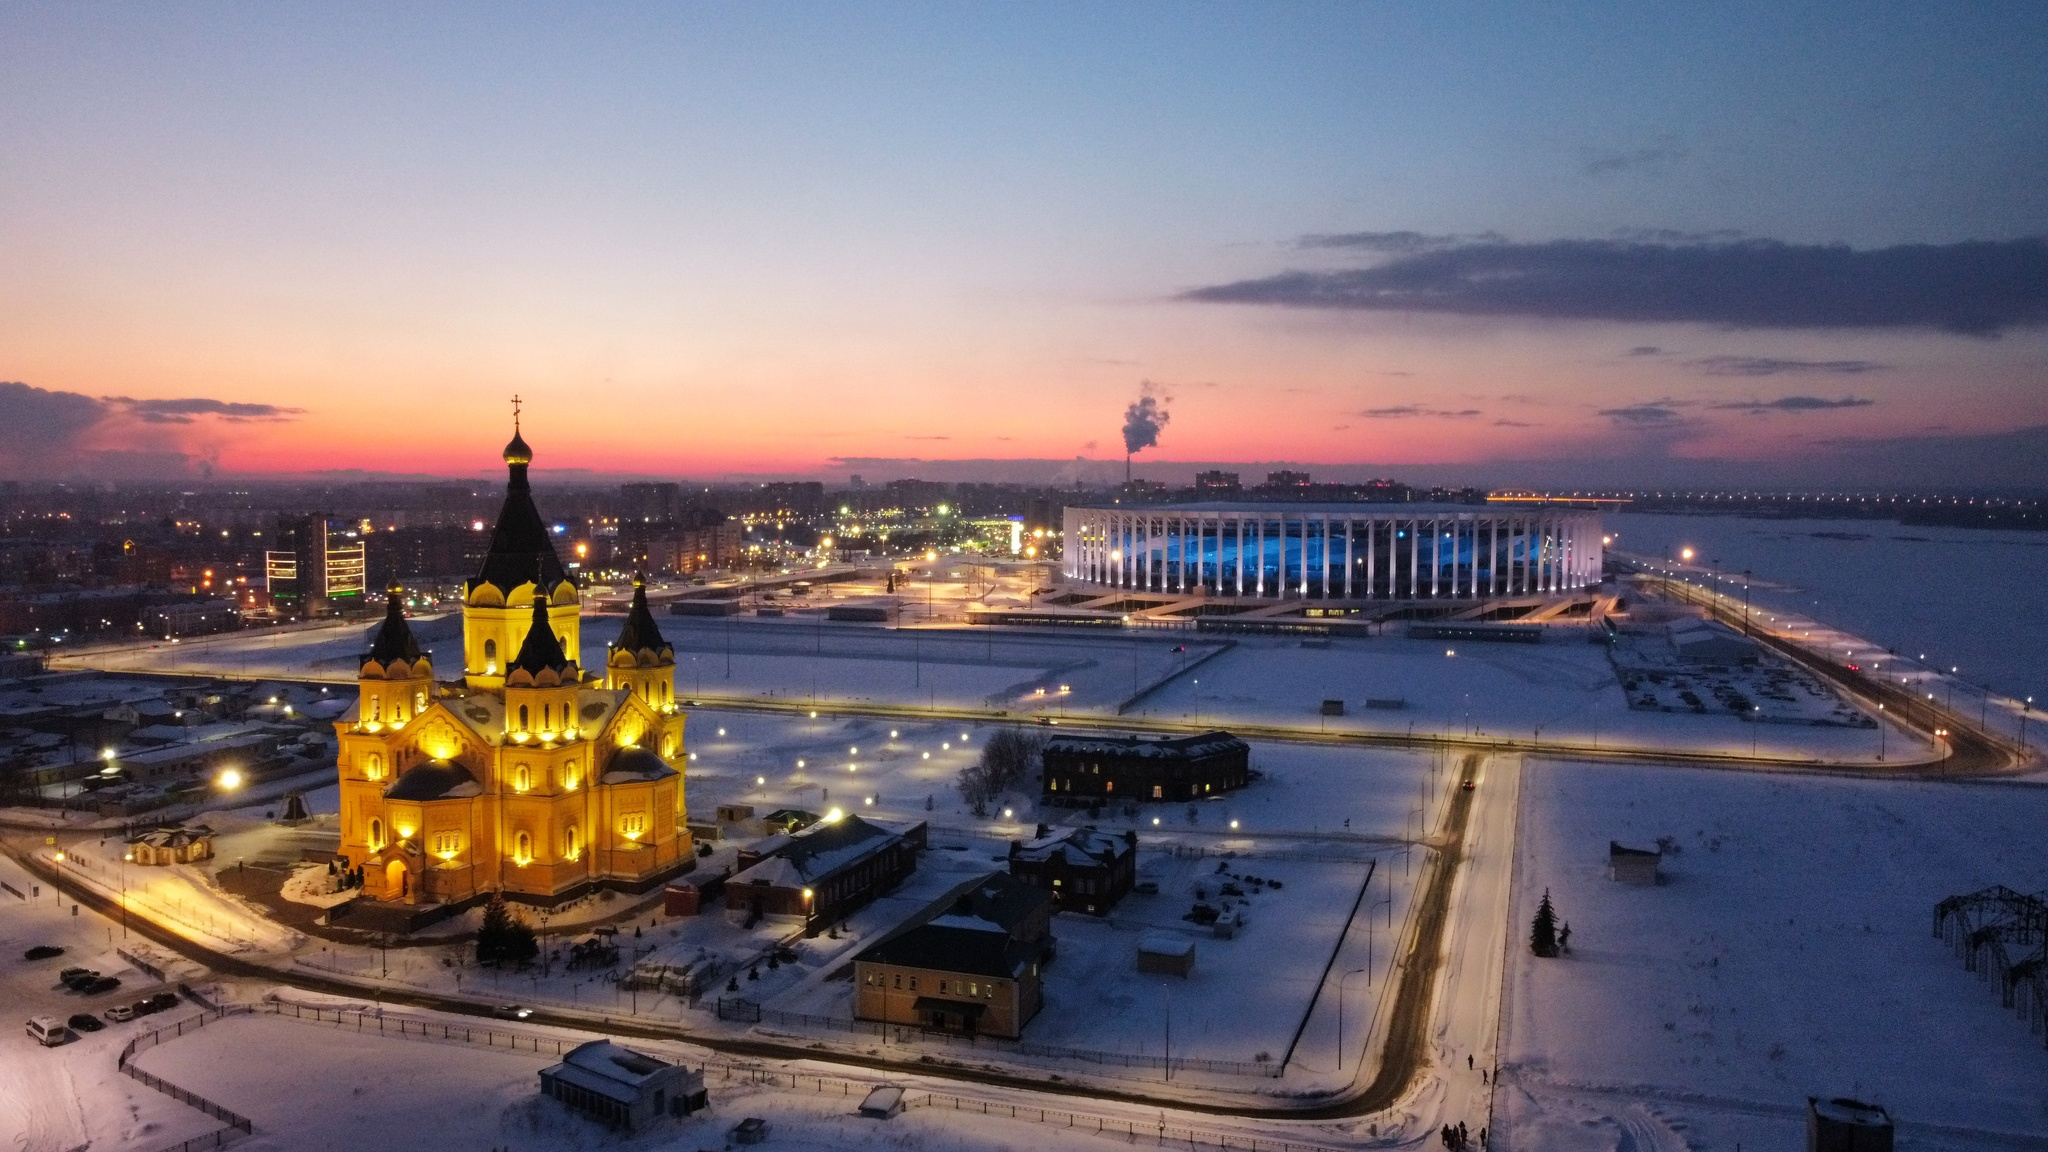
\includegraphics[scale=0.25]{6.png}
        \caption{Интегрирование при $\tau_0 = 5$ мс и $\nu = 5000$ Гц}
        \label{Интегрирование при 5 мс и 5000 Гц}
    \end{figure}
    \item Дифференцирование (рис. \ref{Дифференцирование меандра при 10 мкс и 50 Гц})
    и интегрирование (рис. \ref{Интегрирование меандра при 5 мс и 500 Гц}) меандра,
    соответственно.
    \begin{figure}[h]
        \centering
        \includegraphics[scale=0.25]{7.png}
        \caption{Дифференцирование меандра при $\tau_0 = 10$ мкс и $\nu = 50$ Гц}
        \label{Дифференцирование меандра при 10 мкс и 50 Гц}
    \end{figure}
    \begin{figure}[h]
        \centering
        \includegraphics[scale=0.25]{8.png}
        \caption{Интегрирование меандра при $\tau_0 = 5$ мс и $\nu = 500$ Гц}
        \label{Интегрирование меандра при 5 мс и 500 Гц}
    \end{figure}

    Разложение меандра в ряд Фурье:
    \begin{equation*}
        \dfrac{4}{\pi}\sum\limits_{k=1}^{\infty}\dfrac{sin(\pi  kt)}{k}
    \end{equation*}
    \item Дифференцирование (рис. \ref{Дифференцирование треугольника при 10 мкс и 500 Гц})
    и интегрирование (рис. \ref{Интегрирование треугольника при 5 мс и 500 Гц}) треугольника,
    соответственно.
    \begin{figure}[h]
        \centering
        \includegraphics[scale=0.25]{9.png}
        \caption{Дифференцирование треугольника при $\tau_0 = 10$ мкс и $\nu = 500$ Гц}
        \label{Дифференцирование треугольника при 10 мкс и 500 Гц}
    \end{figure}
    \begin{figure}[h]
        \centering
        \includegraphics[scale=0.25]{10.png}
        \caption{Интегрирование треугольника при $\tau_0 = 5$ мс и $\nu = 500$ Гц}
        \label{Интегрирование треугольника при 5 мс и 500 Гц}
    \end{figure}

    Разложение треугольника в ряд Фурье:
    \begin{equation*}
        \dfrac{8}{\pi^2}\sum\limits_{k=1}^{\infty}(-1)^{\dfrac{k-1}{2}}\dfrac{sin(\pi kt)}{k^2}
    \end{equation*}
    \item Дифференцирование (рис. \ref{Дифференцирование пилы при 10 мкс и 500 Гц})
    и интегрирование (рис. \ref{Интегрирование пилы при 5 мс и 500 Гц}) пилы,
    соответственно.
    \begin{figure}[h]
        \centering
        \includegraphics[scale=0.25]{11.png}
        \caption{Дифференцирование пилы при $\tau_0 = 10$ мкс и $\nu = 500$ Гц}
        \label{Дифференцирование пилы при 10 мкс и 500 Гц}
    \end{figure}
    \begin{figure}[h]
        \centering
        \includegraphics[scale=0.25]{12.png}
        \caption{Интегрирование пилы при $\tau_0 = 5$ мс и $\nu = 500$ Гц}
        \label{Интегрирование пилы при 5 мс и 500 Гц}
    \end{figure}

    Разложение пилы в ряд Фурье:
    \begin{equation*}
        \dfrac{1}{2} - \dfrac{1}{\pi}\sum\limits_{k=1}^{\infty}\dfrac{1}{k}sin(\pi kt)
    \end{equation*}
\end{enumerate}

\end{document}